%%%%%
%%Title: HiPi+Bus V0.2 Chapter 1 Section 4
%%Creator: Ando Ki
%%CreationDate: April 1992
%%FileName: sec3
%%RelatedFile: ch1
%%%%%
\section{블록 구조}

\subsection{관련 블록 간 구조}
시스템 버스 블록(BUS block)은 {\tt <}그림~\ref{figure:block-relation}{\tt >}에서
굵은 선으로 표시된 부분에 해당한다.
%
%
%\documentstyle[11pt,doublespace,a4wide,psfig]{harticle}
%\setstretch{1.2}
%\pagestyle{headings}
%\begin{document}
%
%
\begin{figure}[htb]
%\begin{center}
  \begin{picture}(370,140)(0,-70)
	\thicklines
	\put(40,0){\oval(82,22)} %외곽박스
	\put(40,0){\oval(80,20)\makebox(0,0){시스템버스블록}}
	\put(145,60){\oval(90,20)\makebox(0,0){주처리장치블록}}
	\put(145,30){\oval(90,20)\makebox(0,0){주기억장치블록}}
	\put(145,0){\oval(90,20)\makebox(0,0){입출력처리기블록}}
	\put(145,-30){\oval(90,20)\makebox(0,0){시스템제어기블록}}
	\put(145,-60){\oval(90,20)\makebox(0,0){패키징블록}}
	\put(260,15){\oval(80,20)\makebox(0,0){고장진단블록}}
	\put(260,-15){\oval(80,20)\makebox(0,0){펨웨어블록}}
	\put(360,0){\oval(80,40)}
		\put(360,8){\makebox(0,0){입출력제어기/}}
		\put(360,-9){\makebox(0,0){디바이스블록}}
	\put(80,0){\line(1,3){20}}
	\put(80,0){\line(2,3){20}}
	\put(80,0){\line(1,0){20}}
	\put(80,0){\line(2,-3){20}}
	\put(80,0){\line(1,-3){20}}
	\put(190,60){\line(2,-3){30}}
	\put(190,30){\line(2,-1){30}}
	\put(190,0){\line(2,1){30}}
	\put(190,-30){\line(2,3){30}}
	\put(190,0){\line(2,-1){30}}
	\put(190,-30){\line(2,1){30}}
	\put(250,5){\line(0,-1){10}}
	\put(300,15){\line(2,-1){20}}
	\put(300,-15){\line(2,1){20}}
  \end{picture}
%\end{center}
  \caption{하드웨어 서브시스템의 블록 간 상호관계}\label{figure:block-relation}
\end{figure}
%
%\end{document}
%%%%%

%
즉 하드웨어 서브시스템에서 주 처리 장치 블록(MPU block),
주 기억 장치 블록(MEM block), 입출력 처리기 블록(IOP block), 시스템
제어기 블록(SCM block), 그리고 패키징 블록(PAC block)이 전기적, 기계적, 기능적으로
백플레인에 의해 연결될 때 이 백플레인을
포함한 전기적, 기계적, 기능적 집합체를 시스템 버스 블록이라 한다.

\subsection{시스템의 구성}
공유메모리를 갖는 다중 프로세서 시스템의 시스템 버스인 
\HB는
프로세스, 메모리, 기타 버스 상에 장착되는 보드들 사이의 정보 교환 통로로써 이용된다.
%
\begin{figure}[htb]
    \centerline{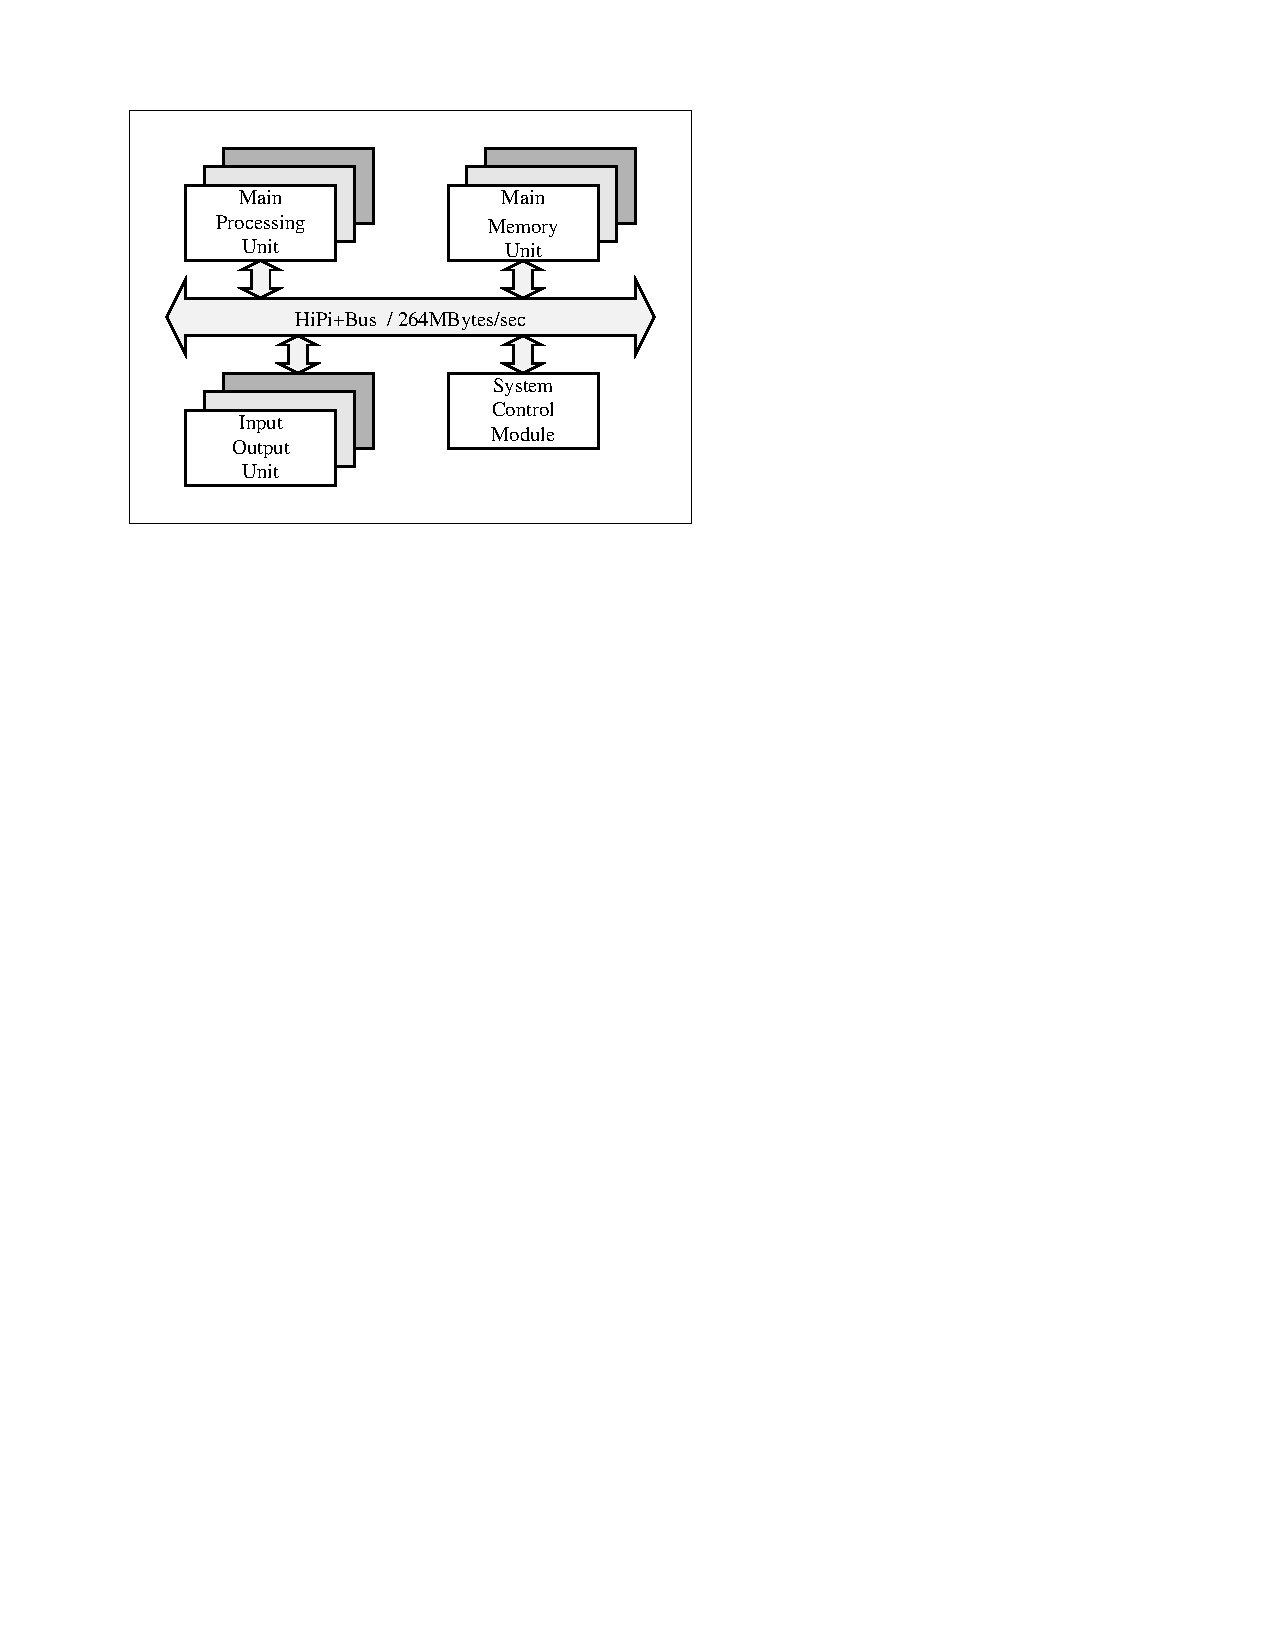
\includegraphics[height=3.5in]{ch1/FIG/system.jpg}} %\centerline{\psfig{figure=ch1/FIG/system.ps,height=3.5in}}
   \caption{시스템 구성}\label{figure:system-config}
\end{figure}
%

\subsection{주요규격}
시스템 버스 블록(BUS block)의 주요규격은 {\tt <}표~\ref{table:bus-spec}{\tt >}와
같다.
%
\begin{table}[htbp]
\caption{\HB의 규격}\label{table:bus-spec}
  \begin{center}
\begingroup
\setlength{\tabcolsep}{6pt} % Default value: 6pt
\renewcommand{\arraystretch}{0.9} % Default value: 1
  \begin{tabular}{|l l|} \hline
   \multicolumn{2}{|c|}{중재 특성 (Characteristics of Arbitration)} \\ \hline
      중재 규칙 & 우선순위와 공정성 (Priority and Fairness) \\
      중재 수행 시간 & 1 Bus Clock (60.6 {\it n\/}sec) \\
      중재 기법 & 선형자가중재 (Linear Self Arbitration) \\
      중재기의 특성 & 분산형 중재기 (Distributed Arbiter) \\
      기타 & Request Inhibition, Request Timeout 구현 \\ \hline
   \multicolumn{2}{|c|}{데이터 전송 특성 (Characteristics of Data Transfer)} \\ \hline
      프로토콜 & 펜디드 (Pended) \\
      제어 방식 & 동기형 (Synchronous) \\
      클럭 속도 & 16.5 MHz (60.6 {\it n\/}sec) \\
      어드레스/데이터 & non-multiplexed \\
      최대 어드레스 영역의 크기 & 4 Gbytes (32 bits wide) \\
      어드레스 영역의 갯수 & 8 (3개 정의) \\
      최대 사용 가능한 전송 형태 & 32 (13개 정의) \\
      버스의 폭 (Bus Width) & 128 bits (16 bytes) \\
      데이터의 단위 (Data Unit) & 8 bits (1 byte) \\
      전송 가능한 데이터의 크기 & 16-바이트 이내의 연속된 바이트; 64-바이트 \\
      정렬의 제약 (Alignment Restriction) & 16 byte boundary; 64 byte boundary \\
      Justification & Straight (Nonjustified) \\
      데이터 전송 속도(Data Transfer Rate) & 264 Mbytes/sec ($16Bytes \times 16.5M\!H\!z$)\\ \hline
   \multicolumn{2}{|c|}{인터럽트 전송 특성 (Characteristics for Interrupt Transfer)} \\ \hline
      전송 프로토콜 & Message passing protocols \\
      제어 방식 & 동기형 (Synchronous) \\
      클럭 속도 & 16.5 MHz (60.6 {\it n\/}sec) \\
      전송 속도 & 최대 약 1.6 MI/sec (Mega Interrupts per second) \\
      중재 기법 & 부호화된 자가중재 (Coded Self Arbitration) \\
      중재기 특성 & 분산형 중재기 (Distributed Arbiter) \\
      에러 방어 & Parity Detection \\
      기타 & Broadcast and Arbitration \\ \hline
    \multicolumn{2}{|c|}{기 타 (Etc.)} \\ \hline
      캐쉬 지원 & Write Back Cache Coherency Protocol \\
      동기화 지원 (Synchronization) & Semaphore Cache Protocol \\
      에러 검출 (Error Detection) & 바이트 단위의 홀수 패리티(odd parity) \\
      에러 처리 (Error Handling) & 재시도 (Retry) \\
      경계주사 (Boundary Scan) & IEEE std.1149.1 \\
      구현 기술 (Technology) & BTL (IEEE std.1194.1) \\
      슬롯 수 & 21 slots/backplane \\
      콘넥터 규격 & 85$\times$4rows (340pins, 전원제외)\\
                  & 40$\times$4rows (160pins, 전원포함)\\
      공급 전원 & +5V, +5V Standby \\
      총 신호수 & 293 (전원제외, 입출력용 제외) \\ \hline
  \end{tabular}
\endgroup
  \end{center}
\end{table}
%


\subsection{블록의 구조}
시스템 버스 블록(BUS block)은 {\tt <}그림~\ref{figure:block}{\tt >}와
같이 크게 중재버스(arbitration bus), 데이터 전송버스(dtat transfer bus),
인터럽트 전송버스(interrupt transfer bus), 그리고 유틸리티 버스(utility bus)로
구분된다.
%
\begin{figure}[htb]
    \centerline{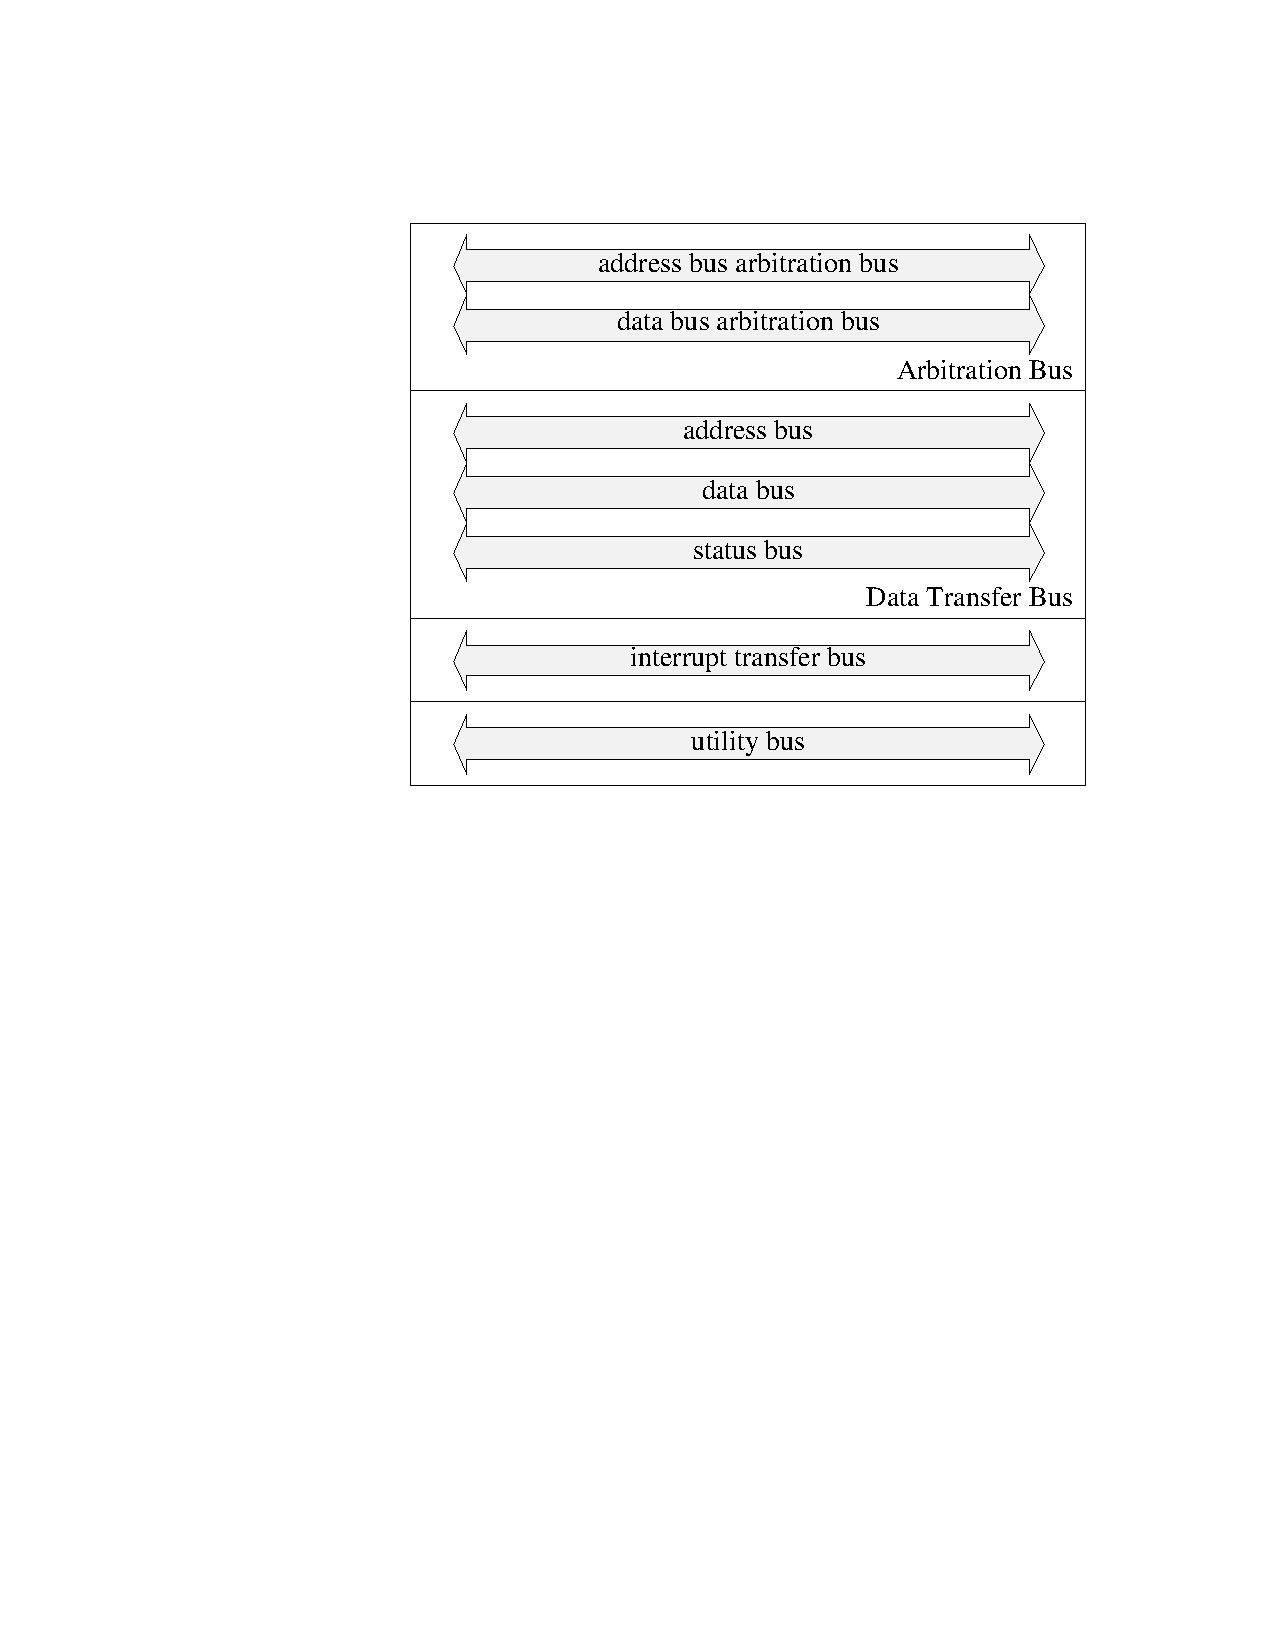
\includegraphics{ch1/FIG/block.jpg}} %\centerline{\psfig{figure=ch1/FIG/block.ps}}
   \caption{버스 블록의 구조}\label{figure:block}
\end{figure}
%
그리고 중재버스는 어드레스 버스 중재버스(address bus arbitration bus)와
데이터 버스 중재버스(data bus arbitration bus)로 구성되고,
데이터 전송버스는 어드레스 버스(address bus), 데이터 버스(data bus),
그리고 상태 버스(status bus)로 구성된다.

\subsection{버스신호들}
시스템 버스에서 정의하여 사용하는 버스 신호들은 {\tt <}표~\ref{table:signals}{\tt >}와
같다.
%\documentstyle[11pt,a4]{hbook}
%\begin{document}
%
\begin{table}[htbp]
\caption{신호선들}\label{table:signals}
   \begin{center}
\begingroup
\setlength{\tabcolsep}{6pt} % Default value: 6pt
\renewcommand{\arraystretch}{0.9} % Default value: 1
   \begin{tabular}{|l|l|r|l|} \hline
Bus&Mnemonic & Size & Name \\ \hline \hline
     & {\bf ABRQ$<$12..0$>$*} & 13 & Address Bus Request \\
     & {\bf ABINH*}                    & 1 & Address Bus Arbitration Inhibition \\
중재버스 & {\bf WRINH*}                    & 1 & Write Cycle Inhibition \\
     & {\bf DBRQ$<$8..0$>$*}  & 9 & Data Bus Request \\
     & {\bf DBINH*}                    & 1 & Data Bus Arbitration Inhibition \\
     & {\bf PCW*}                      & 1 & Priority Change Window \\ \hline
         & {\bf A$<$31..4$>$*}     & 28 & Address \\
         & {\bf AP$<$3..0$>$*}     & 4 & Address Parity \\
         & {\bf SI$<$7..0$>$*}     & 8 & Source Identification \\
         & {\bf SIP*}                      & 1 & Source Identification Parity \\
데이터전송버스  & {\bf AS$<$2..0$>$*}     & 3 & Address Space \\
(어드레스버스) & {\bf TT$<$4..0$>$*}     & 5 & Transfer Types \\
         & {\bf STP*}                      & 1 & Space + Types Parity \\
         & {\bf BE$<$15..0$>$*}    & 16 & Byte Enable \\
         & {\bf BEP$<$1..0$>$*}    & 2 & Byte Enable Parity \\
         & {\bf AE*}                       & 1 & Address Cycle Enable \\ \hline
         & {\bf D$<$127..0$>$*}    & 128 & Data \\
데이터전송버스  & {\bf DP$<$15..0$>$*}    & 16 & Data Parity \\
(데이터버스)  & {\bf DI$<$7..0$>$*}     & 8 & Destination Identification \\
         & {\bf DIP*}                      & 1 & Destination Identification Parity \\
         & {\bf DE*}                       & 1 & Data Cycle Enable \\ \hline
        & {\bf AACK$<$1..0$>$*}   & 2 & Address Acknowledge \\
        & {\bf SHD*}                      & 1 & Hit on Shared Line \\
        & {\bf DTY*}                      & 1 & Hit on Dirty Line \\
데이터전송버스 & {\bf SNK*}                      & 1 & Snoop No Acknowledge \\
(상태버스)  & {\bf ITV*}                      & 1 & Intervention \\
        & {\bf LCR*}                      & 1 & Hit on Interlocked Region \\
        & {\bf DACK*}                     & 1 & Data Acknowledge \\
        & {\bf CDK*}                      & 1 & Cache Data Acknowledge \\
        & {\bf SPIN$<$3..0$>$*}   & 4 & Spin Queue Order \\
        & {\bf BSY$<$7..0$>$*}    & 8 & Busy Status Line \\ \hline    
인터럽트 & {\bf IBSYNC*}                   & 1 & Interrupt Bus Sync. \\
전송버스 & {\bf IBD$<$7..0$>$*}    & 8 & Interrupt Bus Data \\
     & {\bf IBDP*}                     & 1 & Interrupt Bus Data Parity \\ \hline
       & {\bf BCLK*}                   & 1 & Bus Clock \\
유틸리티버스 & {\bf RST*}                      & 1 & System Reset \\
       & {\bf SFAIL*}                    & 1 & System Fail \\
       & {\bf GA$<$4..0$>$*}     & 5 & Geographical Slot Address \\
       & {\bf Tx$<$4..0$>$}     & 5 & JTAG Boundary Scan Option \\ \hline
       & {\it total\/} & 293 & \\
\hline
   \end{tabular}
\endgroup
   \end{center}
\end{table}
%
%\end{document}
%%%%


\subsection{문서 작성의 규칙}

\subsubsection{신호 이름에 대한 규칙}
\begin{itemize}
  \item 버스 신호의 Mnemonics은 모두 대문자를 사용한다. \\
	예: AE*, DE*, A{\tt <}31..4{\tt >}*
  \item 버스 신호의 Mnemonics은 신호 이름 중에서 신호 이름을 대표할 수 있는 앞뒤 몇 문자를 사용한다. \\
	예: Bus Clock : BCLK*; Shared Line : SHD*
  \item 버스 상의 모든 신호의 끝에는 모두 *를 붙힌다. 이는 버스 신호의 전압이 낮은 상태일 때 
	``참 (true)''이 됨을 의미한다. \\
	예: A{\tt <}0{\tt >}*, DTY*
  \item 동일한 이름을 갖는 여러 비트의 신호는 {\tt <}{\tt >}을 사용하여 번호와 크기를 나타낸다. \\
	예: A{\tt <}31..4{\tt >}*,
	A{\tt <}4{\tt >}*, D{\tt <}127..0{\tt >}*, TT{\tt <}3{\tt >}*
  \item 번호는 큰 쪽을 먼저 쓰는 것을 기본(default)으로 한다. \\
	예: A{\tt <}31..4{\tt >}*, D{\tt <}127..0{\tt >}*,
	TT{\tt <}3..0{\tt >}*
  \item 동일 이름을 갖는 여러 비트의 신호중 임의의 한 신호 또는 한 비트를 지칭할 때는 {\tt <}n{\tt >}을 사용한다. \\
	예: A{\tt <}n{\tt >}*, D{\tt <}n{\tt >}*,TT{\tt <}n{\tt >}*
  \item 동일 이름을 갖는 여러 비트의 신호를 총칭할 때는 비트 폭을 모두 표시하거나 또는 비트 폭 표시가 없는
	Mnemonics만으로 표시한다. \\
	예: A{\tt <}31..4{\tt >}* 또는 A*; D{\tt <}127..0{\tt >}* 또는 D*
\end{itemize}
%

\subsubsection{신호의 상태에 대한 규칙}
\begin{itemize}
  \item 신호의 상태는 신호의 논리적인 값(``참''/``거짓'')을 표현하는 방법을 주로 사용하고,
	경우에 따라 버스상에 전압의 높낮음(``high''/``low'')으로 표현하는 방법을 사용한다.
  \item 신호의 논리적인 값을 표현하기 위하여 ``참'', ``거짓'', ``true'', ``false'', 
	T (True의 약자), F (False의 약자), 1, 0을 사용한다.
	``참'', ``true'', T, 1이 같은 값이고, ``거짓'', ``false'', F, 0이 같은 값이다.
	신호의 논리적인 값을 나타낼 때 신호 뒤에 붙는 *는 논리적인 값에 의미를 갖지 않는다. \\
	예: AE* = T, AE = 1, AE* = ``true'', AE* = ``low'', AE* = L : same state \\
	예: DE* = F, DE = 0, DE* = ``false'', DE* = ``high'', DE* = H : same state
  \item 신호의 상태 중 버스 상의 전압 레벨로 표현하기 위하여 ``high'', ``low'', H, L를 사용한다.
	이때 신호의 뒤에 붙는 *는 전압의 레벨를 반대로 하는 역할을 한다. \\
	예: AE* = ``high'', AE* = H, AE = L : same state \\
	예: DE* = ``low'', DE* = L, DE = H : same state
  \item 여러개의 신호가 모여서 의미를 갖는 상태를 나타낼 경우 그 신호의 논리적인
	값은 숫자로 표현할 수 있다. 이때 값의 표현 방법은 
	16진수(Hexadecimal)를 기본(default)으로 한다. \\
	16진수(Hexadecimal)를 나타내는 prefix로 `0x'를 사용한다. \\
	예: A{\tt <}31..4{\tt >}* = 12345,
	TT{\tt <}3..0{\tt >}* = 4, AS{\tt <}3..0{\tt >}* = 0x5
  \item 신호의 상태를 나타낼때 논리적인 값을 사용하는 것을 기본(default)으로 한다. 
	단, 신호의 시간적인 규격을 기술할 때는 전압 레벨을 사용한다(신호의 이름에 
	*의 유무 확인요).
\end{itemize}
%

\subsubsection{시간 규격 표시에 대한 규칙}
\begin{itemize}
  \item 시간 규격은 {\it n\/}sec ($10^{-9}$ 초)를 기본 단위로 한다.
	단, 예외의 경우는 별도로 시간 단위를 표시한다.
  \item 시간 규격에서 사용하는 신호의 타이밍도는 실제 버스에 나타나는 신호를 기준으로 
	설명함을 원칙으로 하고,
	다만 설명의 편의를 위해 구동소자에 관련된 동작을 부가적으로 표시한다.
\end{itemize}
%

\subsubsection{신호의 값을 지정하는 일반적인 규칙}
\begin{itemize}
  \item 신호의 값은 쉽게 구별되도록 지정한다. \\
	예 : TT{\tt <}4..0{\tt >}* 신호에서 TT{\tt <}4{\tt >}*의 값이
	``참(1)''이면 블록에 관련됨을 나타낸다.\\
	예 : TT{\tt <}4..0{\tt >}* 신호에서 TT{\tt <}3{\tt >}*의 값이
	``참(1)''이면 쓰기에 관련됨을 나타낸다.
  \item 응답 신호의 경우 버스에서의 신호의 값이 기본적으로 오류인 것으로 지정한다. \\
	예 : DACK*의 경우 해당 신호의 값을 구동하지 않으면 버스 상에서 전압이 높은 상태로
	유지되므로 자동으로 오류로 값을 갖게 된다.
  \item 신호의 값 중 일부가 {\it don't care\/}인 경우 논리 값이 ``0''이 되게 하여
	버스에서 높은 전압 값을 유지하도록 한다.
\end{itemize}
%%%%%
